\begin{frame}
    \frametitle{Who is behind MISP-LEA?}

    \begin{itemize}
            \item Proposal submitted to the ISF call \textbf{ISF-2022-TF1-AG-CYBER}\footnote{\scriptsize{\url{https://ec.europa.eu/info/funding-tenders/opportunities/docs/2021-2027/isf/wp-call/2021-2022/call-fiche_isf-2022-tf1-ag-cyber_en.pdf}}}
        \item Consortium between \textbf{Shadowserver} and \textbf{CIRCL}
        \item Project start date: \textbf{June 1, 2023}
        \item Project duration: \textbf{24 months}
        \item Objective: Create a sharing hub bridging existing sharing communities and \textbf{Law Enforcement Agencies (LEA)}
    \end{itemize}

    \vspace{1em}

    \begin{figure}
        \centering
        \includegraphics[scale=0.2]{img/misp-lea.png} \\[1em]
        
\includegraphics[scale=0.4]{img/logo-shadowserver.png}
        \hspace{1em}
        
\includegraphics[scale=0.20]{img/logo-circl.pdf}
        \hspace{1em}
        \includegraphics[scale=0.4]{img/eu_funded_en.jpg}
    \end{figure}

\end{frame}

\begin{frame}
\frametitle{MISP-LEA}
\begin{block}{Objectives}
    \begin{itemize}
        \item Operational \textbf{MISP} \& \textbf{AIL} platforms for LEAs.
        \item Operational data feeds from \textbf{CIRCL} \& \textbf{Shadowserver}.
        \item Bridging connections with other operational sharing communities and the private sector.
        \item Platforms are operated by \textbf{CIRCL}.
        \item Main benefit for LEAs: \alert{Bootstrap investigations}.
        \item Enable seamless information sharing with non-EU members.
    \end{itemize}
\end{block}

\begin{block}{Key Figures for 2025}
    \begin{itemize}
        \item Access provided to more than 40 LEA agencies. 121 users.
        \item 2 years of historical data from crawled onion sites, chats,...
    \end{itemize}
\end{block}
\end{frame}

\begin{frame}
    \frametitle{MISP}
    \begin{minipage}{0.45\textwidth} % Adjust width as needed
        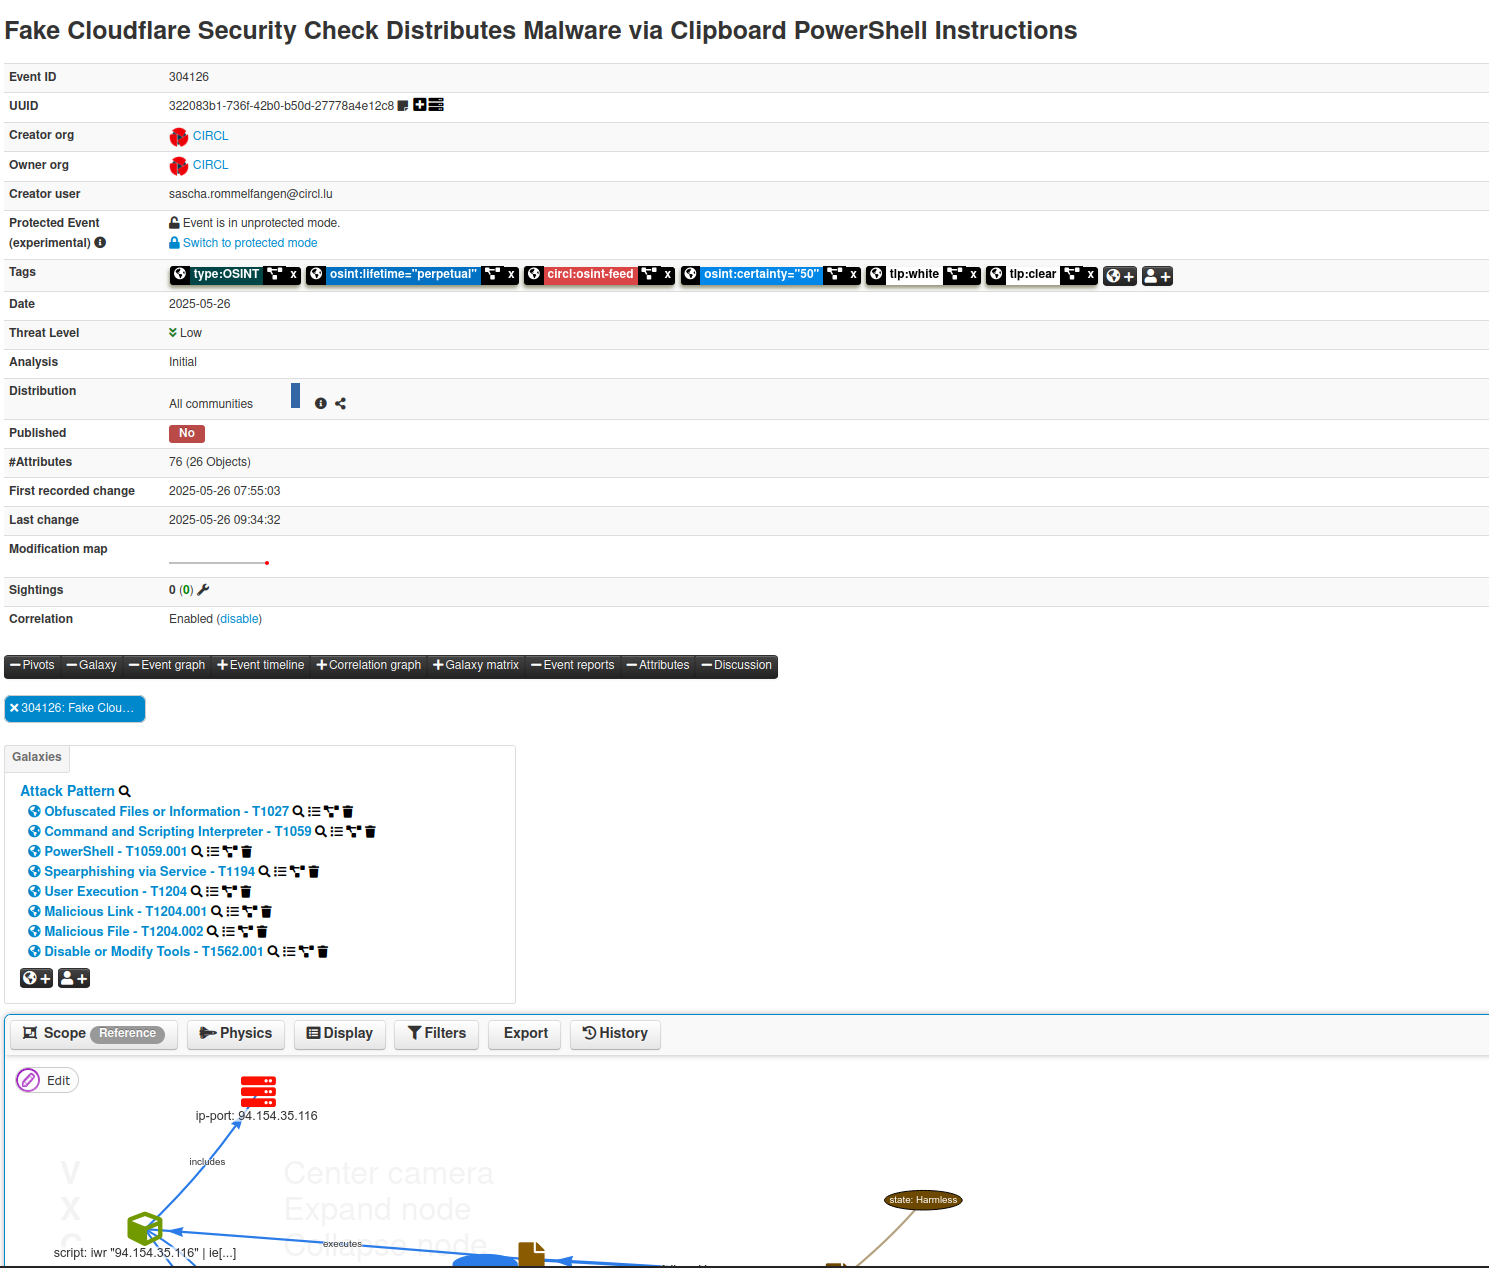
\includegraphics[scale=0.10]{img/misp-scaled.png}
    \end{minipage}%
    \hfill
    \begin{minipage}{0.45\textwidth} % Adjust width as needed
        \begin{itemize}
            \item Foster automated sharing among Law Enforcement Agencies (LEAs).
            \item Establish connections with other sharing communities, such as ISACs and CTI communities.
            \item Share crime indicators that fall outside the scope of CSIRT activities.
        \end{itemize}
    \end{minipage}
\end{frame}

\begin{frame}
    \frametitle{AIL}
    \begin{minipage}{0.45\textwidth} % Adjust width as needed
        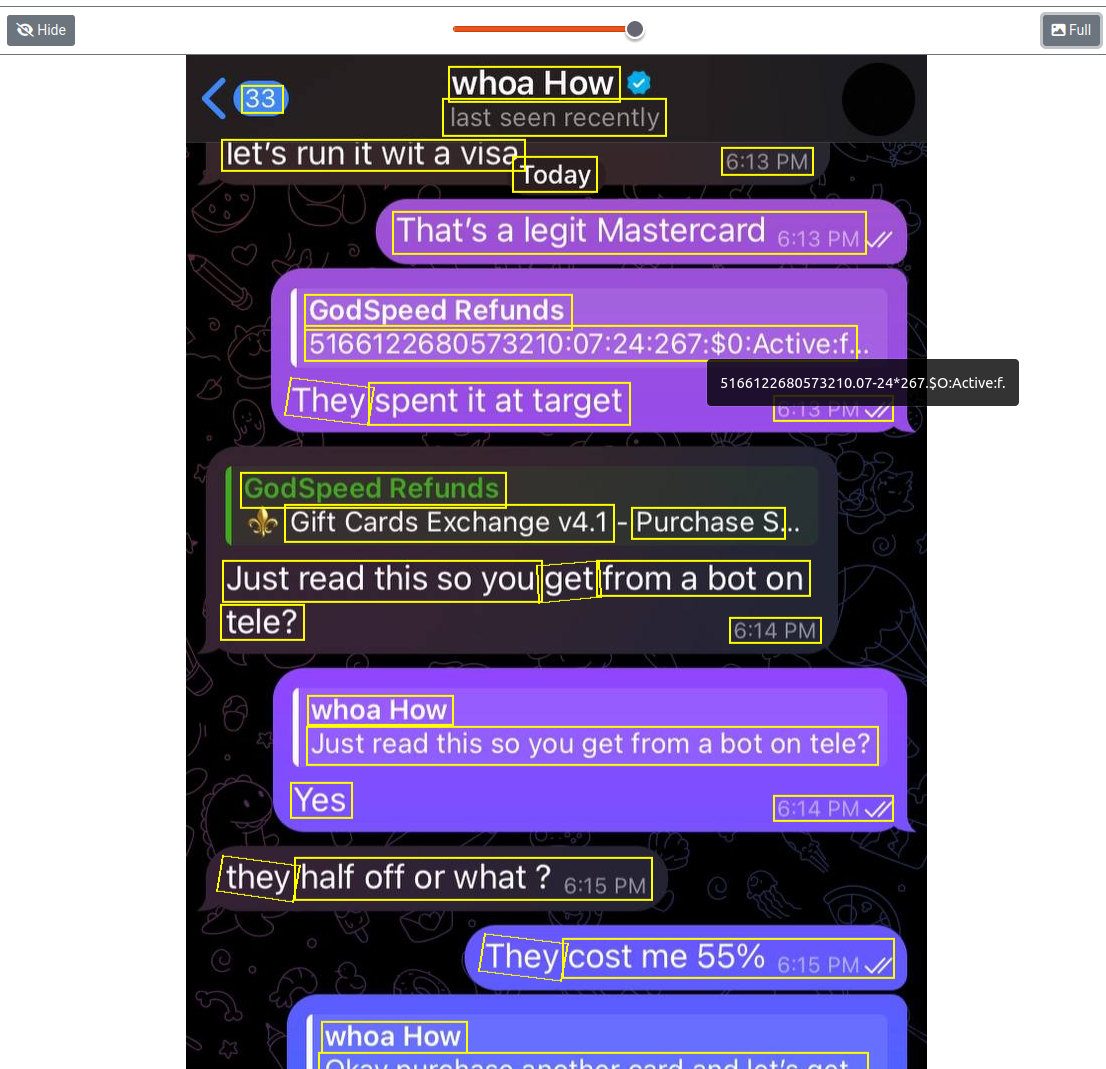
\includegraphics[scale=0.15]{img/ail1.png}
    \end{minipage}%
    \hfill
    \begin{minipage}{0.5\textwidth} % Adjust width as needed
        \begin{itemize}
            \item AIL platform enables the analysis of collected information from various sources.
            \item Focuses on processing data from onion sites, darknet forums, and social media.
            \item Key benefit: Facilitates automated information extraction for investigations.
        \end{itemize}
    \end{minipage}
\end{frame}


